\documentclass[11pt]{article}
\usepackage[final]{acl}

\usepackage{times}
\usepackage{latexsym}
\usepackage[T1]{fontenc}
\usepackage[utf8]{inputenc}
\usepackage{microtype}
\usepackage{graphicx}
\usepackage{booktabs}
\usepackage{amsmath}
\usepackage{url}

\title{SC-LAB at ALTA 2026: Variety-Robust Sentiment and Sarcasm\\
Classification through Per-Cell Ensemble Selection}

\author{
  Author A \quad Author B \quad Author C \quad Author D \quad Author E \\
  SC-LAB, Inje University \\
  \texttt{\{a,b,c,d,e\}@inje.ac.kr}
}

\begin{document}
\maketitle

\begin{abstract}
We present the SC-LAB submission to the ALTA 2026 shared task on joint
sentiment and sarcasm classification for Australian and British English. The
official metric scores each sub-task by its weaker variety, so variety
robustness rather than average accuracy determines the final result. Our
system targets this structure directly: we train a pool of 17 transformer
models, adapt them to the sarcasm domain by intermediate pretraining on 250k
Reddit comments, and combine them using ensemble selection performed
independently for each (task, variety, source) cell, with decision thresholds
fitted on out-of-fold predictions. The system scores \textbf{0.8526} on the
blind test set, and \textbf{0.9304} on the development target, where it ranked
first. We then characterise the relationship between the two evaluation
phases, showing that development scores are optimistic by approximately 0.08
because the protocol permits fitting against a target with public labels,
whereas nested cross-validation predicts blind-test performance to within
0.01. Per-cell ablations identify intermediate pretraining as the dominant
contributor, and we report four negative results on ensembling that we expect
to be useful to future participants.
\end{abstract}

\section{Introduction}

Sentiment classification is a standard sequence-classification problem, but
performance degrades unevenly across national varieties of English. The ALTA
2026 shared task evaluates joint sentiment and sarcasm classification over the
en-AU and en-UK subsets of BESSTIE, drawn from Google Places reviews and
Reddit comments, and scores each sub-task by its \emph{weaker} variety, so a
system that is strong on average but uneven across varieties gains nothing
from its stronger side. We therefore treat the task as four independent
classification problems. Our contributions are:

\begin{itemize}\setlength{\itemsep}{0.1ex}
\item A per-(task, variety, source) ensemble selection procedure with
out-of-fold threshold tuning, which treats each scored cell as its own
optimisation target (\S\ref{sec:system}).
\item A domain-adaptive pretraining study showing that scaling an intermediate
Reddit sarcasm corpus from 60k to 250k examples improves pooled out-of-fold
sarcasm en-UK by 0.037, the single largest gain we measured (\S\ref{sec:dapt}).
\item An analysis of the two evaluation phases demonstrating that
development-phase scores are inflated by approximately 0.08, together with a
nested cross-validation protocol that predicted our blind-test score to within
0.01 (\S\ref{sec:analysis}).
\item Four negative results on ensembling and augmentation, each measured
against a matched baseline (\S\ref{sec:analysis}).
\end{itemize}

\section{Task and Data}

The official metric averages each sub-task's weaker variety:
\begin{equation*}
\begin{aligned}
\text{score} = \tfrac{1}{2}\big(&\min(F_1^{\text{s-AU}}, F_1^{\text{s-UK}})\\
 +\ &\min(F_1^{\text{r-AU}}, F_1^{\text{r-UK}})\big)
\end{aligned}
\end{equation*}
where each $F_1$ is macro-$F_1$ over a (task, variety) cell, s denotes
sentiment and r denotes sarcasm. Capacity spent on a variety that is not the
minimum is wasted, and a single ensemble tuned on pooled accuracy optimises an
average the metric never evaluates. Both observations motivate the per-cell
design in \S\ref{sec:system}.

The data comprises 5{,}531 training and 757 validation rows, with a blind test
release of 1{,}573 rows. Each row carries \texttt{source} (Google or Reddit),
\texttt{variety}, \texttt{text}, and binary \texttt{sentiment} and
\texttt{sarcasm} labels. Both \texttt{source} and \texttt{variety} are
observed at inference time, so conditioning thresholds on them is legitimate.

\begin{table}[t]
\centering\footnotesize
\begin{tabular}{llrrr}
\toprule
source & variety & $n$ & sent.\ pos. & sarc.\ pos. \\
\midrule
google & en-AU & 946 & 0.735 & 0.070 \\
google & en-UK & 1{,}817 & 0.748 & \textbf{0.001} \\
reddit & en-AU & 1{,}763 & 0.319 & 0.419 \\
reddit & en-UK & 1{,}005 & 0.114 & 0.217 \\
\bottomrule
\end{tabular}
\caption{Training class distribution. Sarcasm is near-absent from Google
reviews and effectively nonexistent in google/en-UK ($\approx$2 rows).}
\label{tab:dist}
\end{table}

\begin{figure}[t]
\centering
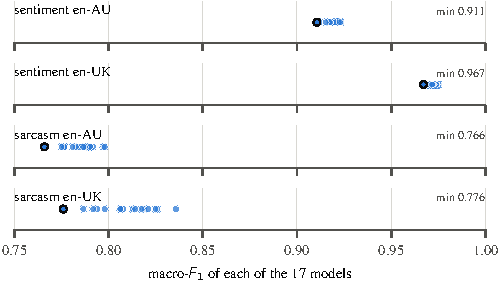
\includegraphics[width=\columnwidth]{fig_cells.pdf}
\caption{Each dot is one of the 17 models on one scored cell; the ringed dot is
that cell's weakest model. Sentiment is tightly clustered and near-solved,
while sarcasm sits 0.13--0.15 lower and is far more dispersed. Because the
metric keeps only the weaker variety per task, the two sarcasm panels decide
the score almost entirely.}
\label{fig:cells}
\end{figure}

Table~\ref{tab:dist} shows the central difficulty. Sarcasm is almost absent
from Google reviews, yet sarcasm-en-UK supplies half the second term of the
score while resting on 218 Reddit positives, so one component of the metric is
determined by a few hundred examples. Figure~\ref{fig:cells} shows the effect
across our pool: sentiment is effectively solved while both sarcasm cells lie
far below it. We additionally observe
$P(\text{negative}\mid\text{sarcastic}) = 96.7\%$ in training, indicating
that annotators recorded intended meaning and that the two tasks are mutually
informative.

\section{System Description}
\label{sec:system}

\subsection{Base Models}

Each model is a shared encoder, mean-pooled over the attention mask, with two
independent 2-class heads trained under a summed loss carrying a tunable
multiplier on the sarcasm term. Every input is prefixed with its
\texttt{source} and \texttt{variety}, both observed at training and test time.
Inputs use head+tail truncation at 192 tokens (75\%/25\%), class-balanced loss
weights, label smoothing of 0.05, multi-sample dropout, and AdamW with
layer-wise learning-rate decay. Encoders are fully fine-tuned; 7--8B decoders
use LoRA adapters \citep{hu2022lora} with $r{=}16$ over 4-bit NF4 weights
\citep{dettmers2023qlora} and last-token pooling. All models use 5-fold
cross-validation stratified jointly on
source~$\times$~variety~$\times$~sentiment~$\times$~sarcasm, so that cells with
single-digit counts cannot fall entirely in one fold.

The final pool of 17 models comprises 14 DeBERTa-v3-large
\citep{he2021deberta} variants (seeds 42/1337/2024; sarcasm-weighted; focal
loss; variety-augmented; and the intermediate-pretraining variants described
below), 2 RoBERTa-large \citep{liu2019roberta}, and Llama-3.1-8B-Instruct
\citep{llama3}.

\subsection{Domain-Adaptive Pretraining}
\label{sec:dapt}

This produced our largest single gain, and is an instance of domain-adaptive
pretraining \citep{gururangan2020}. Every sarcastic row in BESSTIE is a Reddit
comment, but our initial intermediate-task pretraining used news headlines and
tweets --- a domain mismatch on precisely the task that binds the metric. We
built an 847k-row Reddit sarcasm corpus from SARC \citep{khodak2018sarc} and
pretrained the encoder on a 250k balanced subsample before task fine-tuning.
Table~\ref{tab:tapt} compares this against the smaller 60k corpus on matched
fold splits.

\begin{table}[t]
\centering\footnotesize
\begin{tabular}{lrrr}
\toprule
intermediate corpus & r-AU & r-UK & r-UK (OOF) \\
\midrule
60k Reddit, 1 epoch & 0.7837 & 0.8002 & 0.8097 \\
\textbf{250k Reddit, 1 epoch} & \textbf{0.7895} & \textbf{0.8191} & \textbf{0.8463} \\
\bottomrule
\end{tabular}
\caption{Scaling the intermediate pretraining corpus. The first two columns
are fold means; the third is pooled out-of-fold sarcasm macro-$F_1$.}
\label{tab:tapt}
\end{table}

\subsection{Per-Cell Ensemble Selection}

Selection operates on cached out-of-fold probability arrays rather than raw
text, making the search space cheap to explore. Probabilities are
rank-normalised before averaging, since the pool mixes bidirectional encoders
with causal decoders whose probability scales differ (raw-probability
averaging 0.8356 versus rank averaging 0.8670). Each cell receives its own
ensemble, and within a cell each \texttt{source} its own weights and
threshold.

We compared four combination rules, all variants of ensemble selection from a
library of models \citep{caruana2004}: unweighted rank averaging; greedy
subset selection; a weighted blend over an expanded feature space, in which
each model contributes its rank, its raw probability, its cross-task rank and
its inverted rank, with a per-source choice of mean/median/max/min
aggregation; and bagged greedy selection over bootstrap resamples
\citep{caruana2006}.

For the test phase all 17 models were retrained on the union of the training
and validation splits (6{,}288 rows, $+$14\% data, raising en-UK sarcasm
positives from 218 to 248), and every weight, aggregation and threshold was
fitted on out-of-fold predictions only.

\begin{figure}[t]
\centering
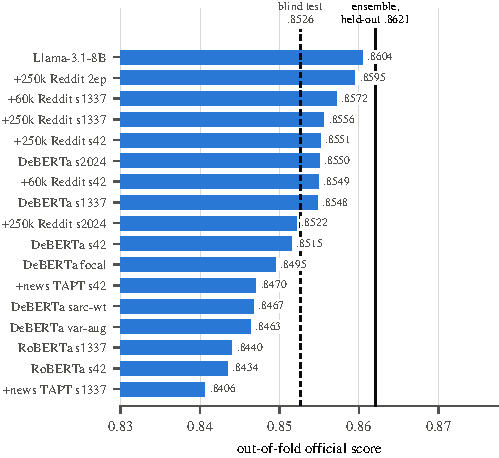
\includegraphics[width=\columnwidth]{fig_pool.pdf}
\caption{All 17 pool members, out-of-fold over the 6{,}288-row pool at a fixed
0.5 threshold, against the ensemble built from them. The best single model
(.8604) reaches within .0017 of the ensemble's held-out estimate and exceeds
its realised blind-test score: combination contributes far less here than
model quality does.}
\label{fig:pool}
\end{figure}

\section{Results}

\subsection{Development Phase}

Under the task's development protocol, ensemble weights and thresholds may be
fitted against the 757-row development target. Table~\ref{tab:dev} reports our
submission and its improvement.

\begin{table}[t]
\centering\footnotesize
\setlength{\tabcolsep}{3.2pt}
\begin{tabular}{lrrrrr}
\toprule
system & s-AU & s-UK & r-AU & r-UK & score \\
\midrule
expanded blend & .9566 & .9870 & .8934 & .8978 & .9250 \\
\,+ re-opt.\ sent. & \textbf{.9675} & \textbf{.9948} & .8934 & .8978 & \textbf{.9304} \\
\bottomrule
\end{tabular}
\caption{Development-phase results, fitted against the development target and
scored on that same target.}
\label{tab:dev}
\end{table}

A later 2{,}000-restart search raised sarcasm-en-UK to 0.9123 but left the
binding sarcasm-en-AU cell at 0.8934, so the final score did not move at all
--- a direct demonstration that only the argmin matters.

\subsection{Test Phase}

All weights and thresholds were fitted on out-of-fold predictions. The
held-out column of Table~\ref{tab:test} is nested cross-validation: the blend
is selected on 4/5 of the out-of-fold rows and scored on the withheld 1/5.

\begin{table}[t]
\centering\footnotesize
\setlength{\tabcolsep}{4pt}
\begin{tabular}{lrrr}
\toprule
combination rule & held-out & in-samp. & gap \\
\midrule
rank averaging & .8568 {\scriptsize$\pm$.0037} & .8629 & .006 \\
\textbf{greedy subset} & \textbf{.8621} {\scriptsize$\pm$.0076} & .8753 & .013 \\
bagged greedy & .8615 {\scriptsize$\pm$.0050} & --- & --- \\
expanded blend & .8578 {\scriptsize$\pm$.0067} & .8788 & .021 \\
\bottomrule
\end{tabular}
\caption{Test-phase combination rules, all fitted on out-of-fold predictions
with no access to test labels.}
\label{tab:test}
\end{table}

We submitted greedy subset selection. It scored \textbf{0.8526} on the blind
test set, placing 6th. Our pre-submission estimate was 0.8621, so the
prediction was accurate to 0.0095 --- consistent with ordinary selection
optimism.

\section{Discussion}
\label{sec:analysis}

\paragraph{Development scores are inflated by $\approx$0.08.}
Development submissions are scored against a file whose gold labels are
distributed with the public data, so fitting ensemble weights and thresholds
against it measures training fit rather than generalisation. Our 0.9304 was
obtained under that protocol; the identical pipeline refitted on out-of-fold
predictions scores 0.8526 on blind data. A simple diagnostic detects the
effect: our best development-phase sarcasm cell (0.8329) exceeds the
oracle-on-target ceiling of every individual pool member (0.8162), which is
unattainable without target information. We recommend that future editions
either withhold development labels or report a held-out estimate alongside the
leaderboard figure.

\paragraph{Nested cross-validation is well calibrated.}
It predicted 0.8621 against a realised 0.8526. In-sample scores are not
predictive: the expanded-feature blend attains the best in-sample score
(0.8788) and the second-worst held-out score, a gap of 0.021
(Table~\ref{tab:test}).

\paragraph{Effective components.}
Scaling intermediate pretraining contributes most ($+$0.037 pooled
out-of-fold on sarcasm-en-UK), followed by per-cell ensembling. Two models
with unremarkable aggregate scores carry the largest weight in specific
cells, confirming that members must be assessed per cell. Restricting
sarcasm-specialised members to the sarcasm cells is necessary: including them
in all four regresses sentiment-en-AU from 0.9321 to 0.9266 and cancels the
sarcasm gain.

\paragraph{Negative results.}
The following were measured against matched baselines and rejected. \emph{Variety-invariance
augmentation}: randomly neutralising the variety token to force a single
shared detector, motivated by en-UK having 218 sarcastic training rows against
en-AU's 739, gave out-of-fold sarc-AU $0.7896\!\rightarrow\!0.7767$ and
sarc-UK $0.8160\!\rightarrow\!0.8140$ --- worse on both, refuting the
hypothesis. \emph{Bagged selection}, the one methodological gap in our
submitted rule, changed nothing (0.8615 versus 0.8621), indicating the
variance was not in the selection step. \emph{Prior-matched quantile
thresholding} (0.8537) and \emph{logistic stacking} with a cross-task
sentiment feature (0.8591) both fell below plain argmax thresholding (0.8611).
\emph{A second seed} of our best pretrained model collapsed sarc-UK to 0.7553:
with roughly 30 validation positives deciding that cell, adding correlated
members is actively dangerous.

\paragraph{Ensembling saturated.}
Across five combination rules the held-out spread was only 0.0053, and
pairwise disagreement between their test-set predictions was 1\% for sentiment
and 3--4\% for sarcasm. As Figure~\ref{fig:pool} shows, the best single model
(0.8604 out-of-fold) came within 0.0017 of the full 17-model blend's held-out
estimate and in fact exceeded its realised blind-test score. The remaining
headroom is in the base models, not the combiner.

\section{Practical Considerations}

Training is sensitive to library versions in a way that produces no error
signal. Under Python 3.13 with PyTorch 2.12 and Transformers 5.11,
DeBERTa-v3-large diverges: training loss \emph{rises} from 1.28 to 1.42,
chance level for two binary tasks, whereas under Python 3.8 with PyTorch 2.1.2
and Transformers 4.46.3 it falls from 0.99 to 0.50 on identical data, seed and
hardware. No exception or warning is raised. The older environment, however,
cannot load Qwen3 (which requires Transformers $\geq$\,4.51) and rejects
Phi-4-mini's \texttt{rope\_scaling} configuration, so the pool composition is
itself constrained by the environment. We therefore pin the training
environment and assert that first-epoch loss falls below a known-good
threshold before committing compute to a full run.

\section{Conclusion}

We described a per-cell ensemble system for variety-robust sentiment and
sarcasm classification, scoring 0.8526 on the ALTA 2026 blind test set and
0.9304 on the development target. Domain-adaptive pretraining on Reddit
sarcasm is the largest single contributor. We showed that development and
blind-test scores are not comparable under this task's protocol, and that
nested cross-validation closes the gap to 0.01. Since five combination rules
span only 0.005 while the best single model nearly matches the full ensemble,
we expect further gains to come from stronger base models and from the
$\approx$250 en-UK sarcasm positives that determine the binding cell, rather
than from the combiner.

{\small
\bibliography{custom}
}

\end{document}
